Айоу, АКа, вот вам ... картинка с гугл диска, которая мне очень приглянулась.

\begin{figure}[ht!]
    \centering
    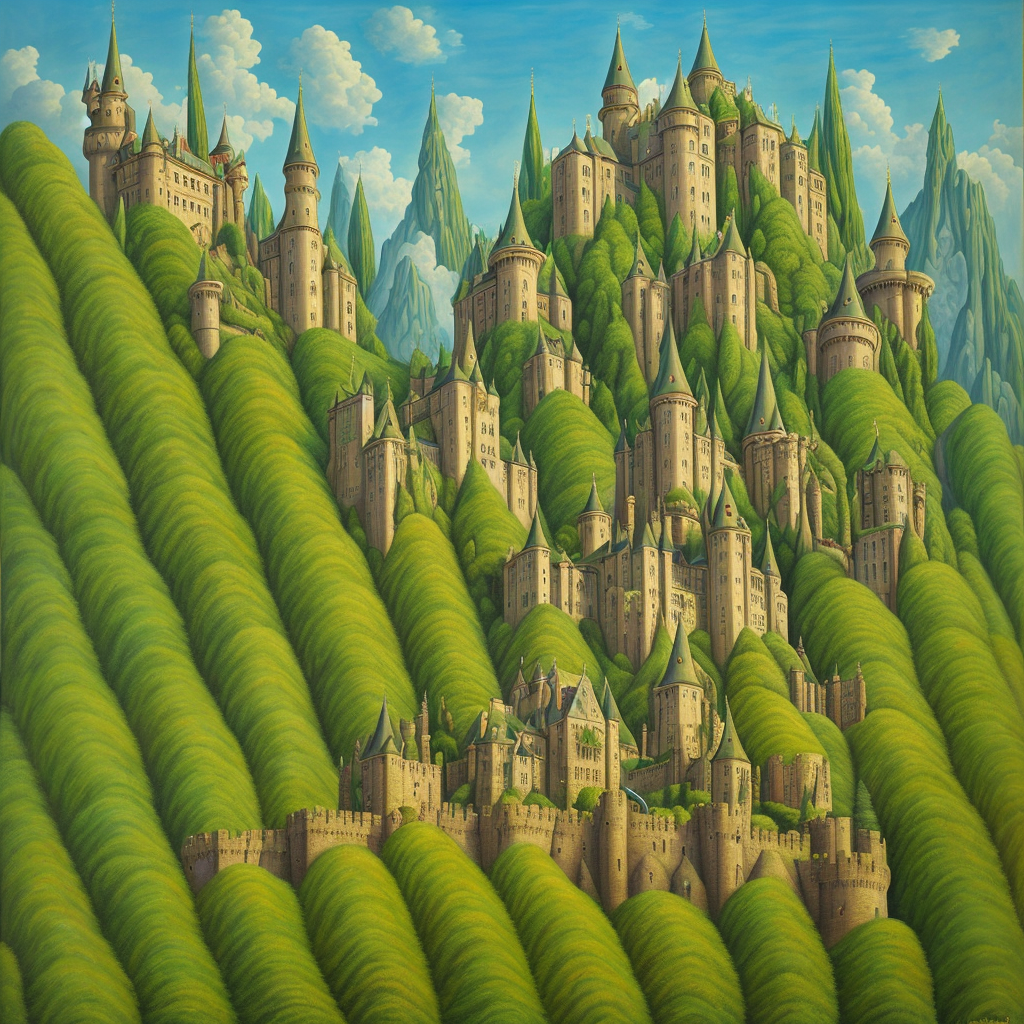
\includegraphics[width=1\textwidth]{/Users/nikolajprovorov/Yandex.Disk-368690@edu.itmo.ru.localized/Lab6_Furry_series/7.png}
    \caption{Картинка с гугл диска, которая мне очень приглянулась.}
    \label{fig:Source_img_1}
\end{figure}

Дальше по инструкции, работаем как сказано, но переписываем код под Python.

А вот и результат, мы получили фурье-образ изображения.

\begin{figure}[ht!]
    \centering
    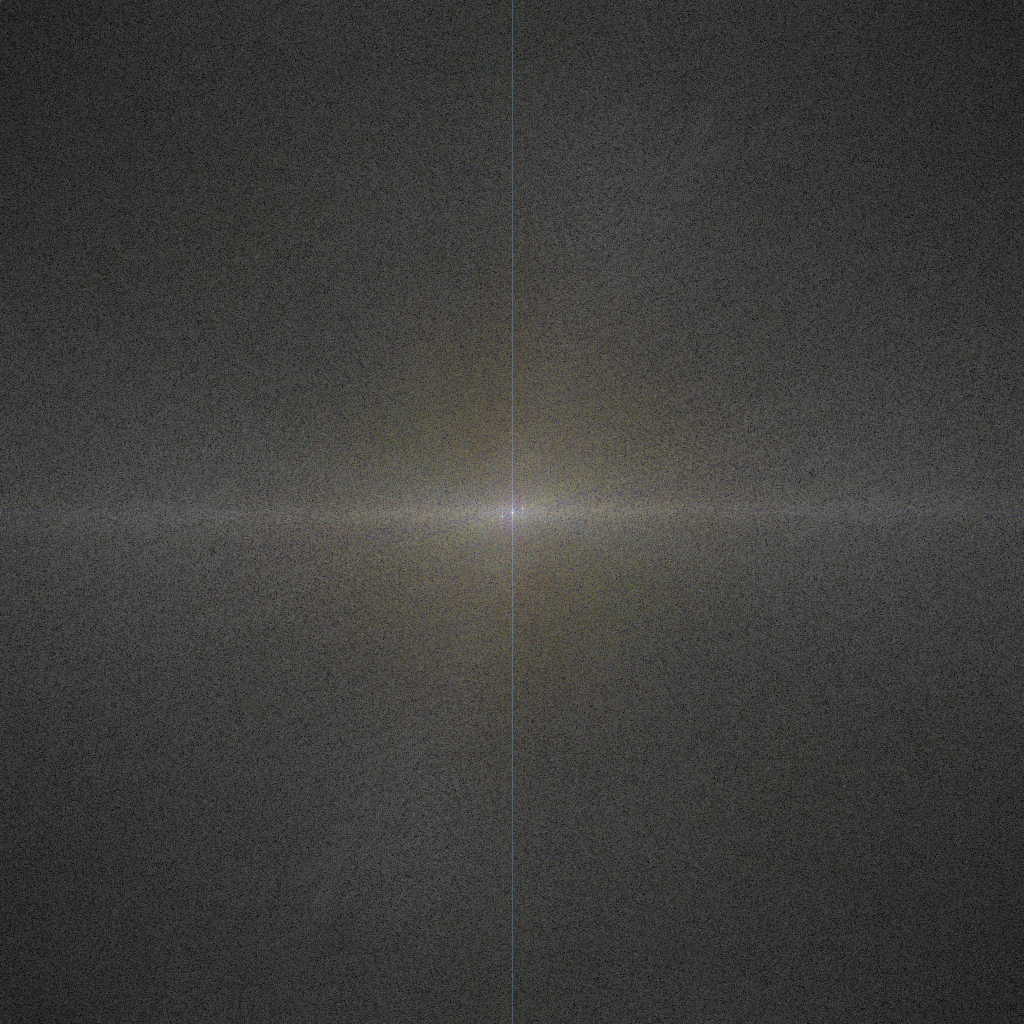
\includegraphics[width=1\textwidth]{/Users/nikolajprovorov/Yandex.Disk-368690@edu.itmo.ru.localized/Lab6_Furry_series/abs_fourier_log.png}
    \caption{Фурье-образ изображения.}
\end{figure}

\clearpage

На изображении присутсвует периодичность, которую мы можем убрать, если убрать пики. А вот и они:

\begin{figure}[ht!]
    \centering
    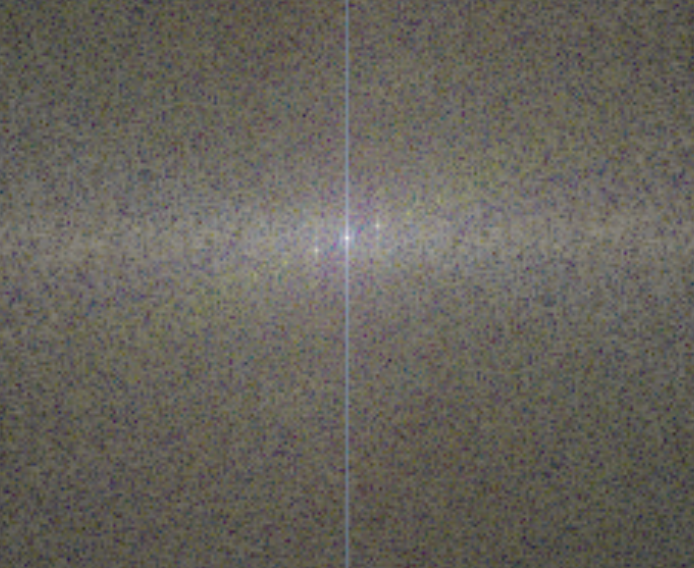
\includegraphics[width=1\textwidth]{/Users/nikolajprovorov/Yandex.Disk-368690@edu.itmo.ru.localized/Lab6_Furry_series/image.png}
    \caption{Пики.}
\end{figure}

Убрали в фотошопе, а вот и результат:

\clearpage

\begin{figure}[ht!]
    \centering
    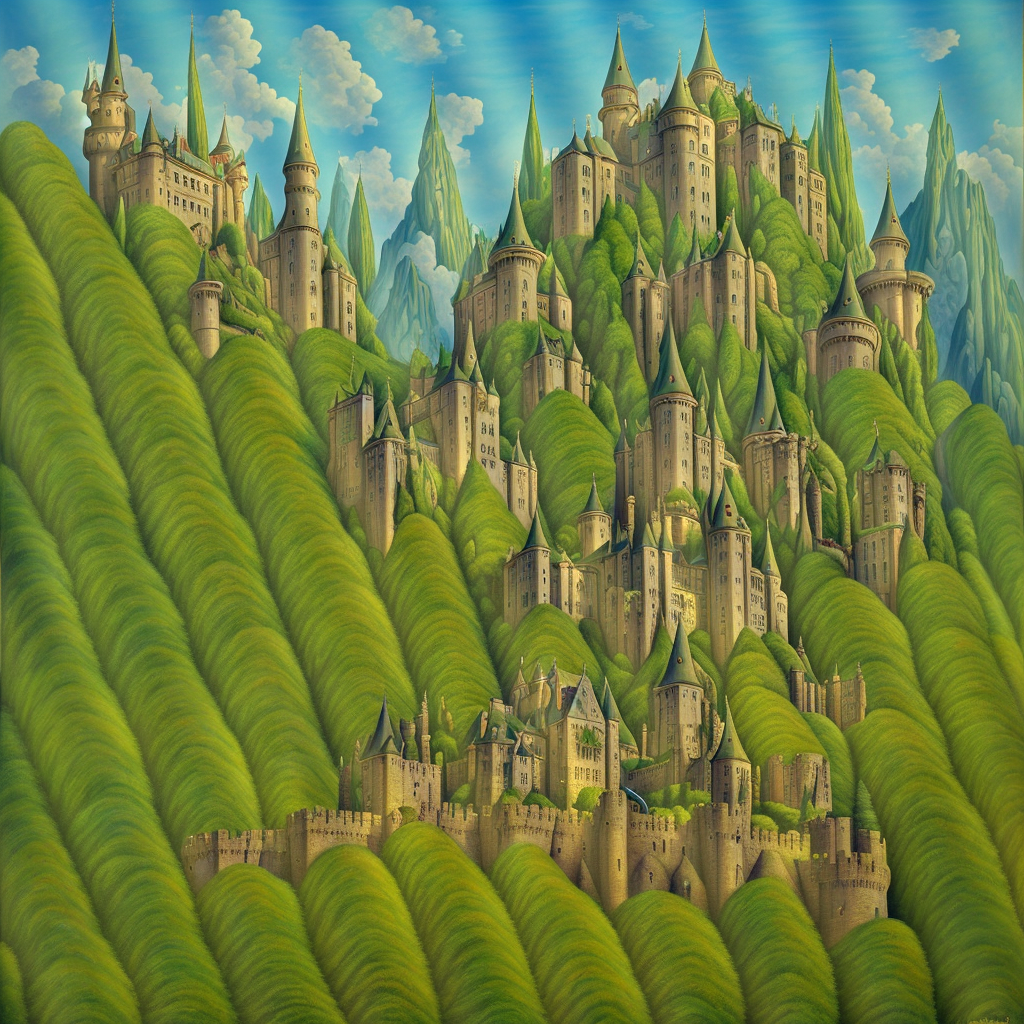
\includegraphics[width=1\textwidth]{/Users/nikolajprovorov/Yandex.Disk-368690@edu.itmo.ru.localized/Lab6_Furry_series/restored.png}
    \caption{Результат.}
\end{figure}

Стало лучше, и мне это нравится. Чуть изменилось само изображение, возможно мы затронули то, что не надо было, но уже ладно. Двигаемся дальше.

